%%%% Paramétrage du TD %%%%
\def\xxactivite{Colle \ifprof -- Corrigé \else \fi} % \normalsize \vspace{-.4cm}
\def\xxauteur{\textsl{Xavier Pessoles}}


\def\xxnumchapitre{Chapitre 1 \vspace{.2cm}}
\def\xxchapitre{\hspace{.12cm} Correction des systèmes}


\def\xxcompetences{%
\vspace{-.3cm}
\textsl{%
\textbf{Savoirs et compétences :}\\
\vspace{-.4cm}
\begin{itemize}[label=\ding{112},font=\color{ocre}] 
%\item \textit{Res1.C4 : } Correction
 \item \textit{Res1.C4.SF1 : } Proposer la démarche de réglage d’un correcteur proportionnel
%proportionnel intégral 
%et à avance de phase
\item \textit{Con.C2 : } 	Correction d’un système asservi	
\item \textit{Con.C2.SF1 : } Choisir un type de correcteur adapté
\end{itemize}
}}

\def\xxauteur{\textsl{Xavier Pessoles}}

\def\xxtitreexo{Système mobile d’imagerie interventionnelle Discovery IGS 730 \ifnormal $\star$ \else \fi \iftdifficile $\star\star\star$ \else \fi }
\def\xxsourceexo{\hspace{.2cm} \footnotesize{Concours CCINP -- MP 2018}}

\def\xxfigures{
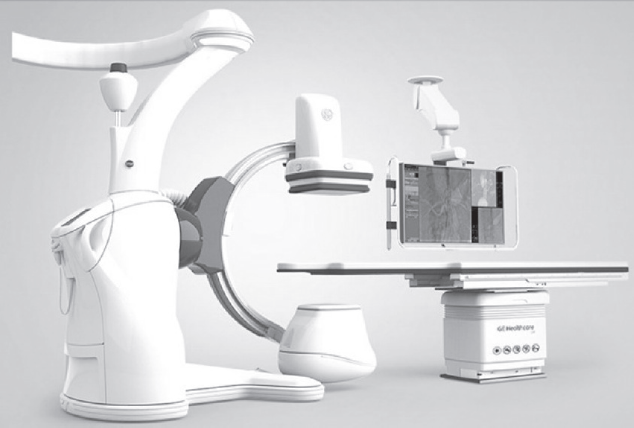
\includegraphics[width=.6\linewidth]{images/ccp_00}
}%figues de la page de garde


\iflivret
\pagestyle{empty}


%%%%%%%% PAGE DE GARDE COURS
\ifcours
\begin{tikzpicture}[remember picture,overlay]
\node at (current page.north west)
{\begin{tikzpicture}[remember picture,overlay]
\node[anchor=north west,inner sep=0pt] at (0,0) {\includegraphics[width=\paperwidth]{\thechapterimage}};
\draw[anchor=west] (-2cm,-8cm) node [line width=2pt,rounded corners=15pt,draw=ocre,fill=white,fill opacity=0.6,inner sep=40pt]{\strut\makebox[22cm]{}};
\draw[anchor=west] (1cm,-8cm) node {\huge\sffamily\bfseries\color{black} %
\begin{minipage}{1cm}
\rotatebox{90}{\LARGE\sffamily\textsc{\color{ocre}\textbf{\xxnumpartie}}}
\end{minipage} \hfill
\begin{minipage}[c]{14cm}
\begin{titrepartie}
\begin{flushright}
\renewcommand{\baselinestretch}{1.1} 
\Large\sffamily\textsc{\textbf{\xxpartie}}
\renewcommand{\baselinestretch}{1} 
\end{flushright}
\end{titrepartie}
\end{minipage} \hfill
\begin{minipage}[c]{3.5cm}
{\large\sffamily\textsc{\textbf{\color{ocre} \discipline}}}
\end{minipage} 
 };
\end{tikzpicture}};
\end{tikzpicture}


\begin{tikzpicture}[overlay]
\node[shape=rectangle, 
      rounded corners = .25 cm,
	  draw= ocre,
	  line width=2pt, 
	  fill = ocre!10,
	  minimum width  = 2.5cm,
	  minimum height = 3cm,] at (18cm,0) {};
\node at (17.7cm,0) {\rotatebox{90}{\textbf{\Large\color{ocre}{\classe}}}};
%{};
\end{tikzpicture}

\vspace{3.5cm}

\begin{tikzpicture}[remember picture,overlay]
\draw[anchor=west] (-2cm,-6cm) node {\huge\sffamily\bfseries\color{black} %
\begin{minipage}{2cm}
\begin{center}
\LARGE\sffamily\textsc{\color{ocre}\textbf{\xxactivite}}
\end{center}
\end{minipage} \hfill
\begin{minipage}[c]{15cm}
\begin{titrechapitre}
\renewcommand{\baselinestretch}{1.1} 
\Large\sffamily\textsc{\textbf{\xxnumchapitre}}

\Large\sffamily\textsc{\textbf{\xxchapitre}}
\vspace{.5cm}

\renewcommand{\baselinestretch}{1} 
\normalsize\normalfont
\xxcompetences
\end{titrechapitre}
\end{minipage}  };
\end{tikzpicture}
\vfill

\begin{flushright}
\begin{minipage}[c]{.3\linewidth}
\begin{center}
\xxfigures
\end{center}
\end{minipage}\hfill
\begin{minipage}[c]{.6\linewidth}
\startcontents
\printcontents{}{1}{}
\end{minipage}
\end{flushright}

\begin{tikzpicture}[remember picture,overlay]
\draw[anchor=west] (4.5cm,-.7cm) node {
\begin{minipage}[c]{.2\linewidth}
\begin{flushright}

\includegraphics[width=2cm]{png/logoCC}
\end{flushright}
\end{minipage}
\begin{minipage}[c]{.2\linewidth}
\textsl{\xxauteur} \\
\textsl{\classe}
\end{minipage}
 };
\end{tikzpicture}
\newpage
\pagestyle{fancy}

\newpage
\pagestyle{fancy}

\else
\fi


%%%%%%%% PAGE DE GARDE TD
\iftd
%\begin{tikzpicture}[remember picture,overlay]
%\node at (current page.north west)
%{\begin{tikzpicture}[remember picture,overlay]
%\draw[anchor=west] (-2cm,-3.25cm) node [line width=2pt,rounded corners=15pt,draw=ocre,fill=white,fill opacity=0.6,inner sep=40pt]{\strut\makebox[22cm]{}};
%\draw[anchor=west] (1cm,-3.25cm) node {\huge\sffamily\bfseries\color{black} %
%\begin{minipage}{1cm}
%\rotatebox{90}{\LARGE\sffamily\textsc{\color{ocre}\textbf{\xxnumpartie}}}
%\end{minipage} \hfill
%\begin{minipage}[c]{13.5cm}
%\begin{titrepartie}
%\begin{flushright}
%\renewcommand{\baselinestretch}{1.1} 
%\Large\sffamily\textsc{\textbf{\xxpartie}}
%\renewcommand{\baselinestretch}{1} 
%\end{flushright}
%\end{titrepartie}
%\end{minipage} \hfill
%\begin{minipage}[c]{3.5cm}
%{\large\sffamily\textsc{\textbf{\color{ocre} \discipline}}}
%\end{minipage} 
% };
%\end{tikzpicture}};
%\end{tikzpicture}

%%%%%%%%%% PAGE DE GARDE TD %%%%%%%%%%%%%%%
%\begin{tikzpicture}[overlay]
%\node[shape=rectangle, 
%      rounded corners = .25 cm,
%	  draw= ocre,
%	  line width=2pt, 
%	  fill = ocre!10,
%	  minimum width  = 2.5cm,
%	  minimum height = 2.5cm,] at (18.5cm,0) {};
%\node at (17.7cm,0) {\rotatebox{90}{\textbf{\Large\color{ocre}{\classe}}}};
%%{};
%\end{tikzpicture}

% PARTIE ET CHAPITRE
%\begin{tikzpicture}[remember picture,overlay]
%\draw[anchor=west] (-1cm,-2.1cm) node {\large\sffamily\bfseries\color{black} %
%\begin{minipage}[c]{15cm}
%\begin{flushleft}
%\xxnumchapitre \\
%\xxchapitre
%\end{flushleft}
%\end{minipage}  };
%\end{tikzpicture}

% Bandeau titre exo
\begin{tikzpicture}[remember picture,overlay]
\draw[anchor=west] (-2cm,-4cm) node {\huge\sffamily\bfseries\color{black} %
\begin{minipage}{5cm}
\begin{center}
\LARGE\sffamily\color{ocre}\textbf{\textsc{\xxactivite}}

\begin{center}
\xxfigures
\end{center}

\end{center}
\end{minipage} \hfill
\begin{minipage}[c]{12cm}
\begin{titrechapitre}
\renewcommand{\baselinestretch}{1.1} 
\large\sffamily\textbf{\textsc{\xxtitreexo}}

\small\sffamily{\textbf{\textit{\color{black!70}\xxsourceexo}}}
\vspace{.5cm}

\renewcommand{\baselinestretch}{1} 
\normalsize\normalfont
\xxcompetences
\end{titrechapitre}
\end{minipage}  };
\end{tikzpicture}

\else
\fi


%%%%%%%% PAGE DE GARDE FICHE
\iffiche
\begin{tikzpicture}[remember picture,overlay]
\node at (current page.north west)
{\begin{tikzpicture}[remember picture,overlay]
\draw[anchor=west] (-2cm,-3.25cm) node [line width=2pt,rounded corners=15pt,draw=ocre,fill=white,fill opacity=0.6,inner sep=40pt]{\strut\makebox[22cm]{}};
\draw[anchor=west] (1cm,-3.25cm) node {\huge\sffamily\bfseries\color{black} %
\begin{minipage}{1cm}
\rotatebox{90}{\LARGE\sffamily\textsc{\color{ocre}\textbf{\xxnumpartie}}}
\end{minipage} \hfill
\begin{minipage}[c]{14cm}
\begin{titrepartie}
\begin{flushright}
\renewcommand{\baselinestretch}{1.1} 
\large\sffamily\textsc{\textbf{\xxpartie} \\} 

\vspace{.2cm}

\normalsize\sffamily\textsc{\textbf{\xxnumchapitre -- \xxchapitre}}
\renewcommand{\baselinestretch}{1} 
\end{flushright}
\end{titrepartie}
\end{minipage} \hfill
\begin{minipage}[c]{3.5cm}
{\large\sffamily\textsc{\textbf{\color{ocre} \discipline}}}
\end{minipage} 
 };
\end{tikzpicture}};
\end{tikzpicture}


\begin{tikzpicture}[overlay]
\node[shape=rectangle, 
      rounded corners = .25 cm,
	  draw= ocre,
	  line width=2pt, 
	  fill = ocre!10,
	  minimum width  = 2.5cm,
	  minimum height = 2.5cm,] at (18.5cm,0.5cm) {};
%	  minimum height = 2.5cm,] at (18.5cm,0cm) {};
\node at (17.7cm,0.5) {\rotatebox{90}{\textsf{\textbf{\large\color{ocre}{\classe}}}}};
%{};
\end{tikzpicture}



\else
\fi



\else
\pagestyle{empty}


%%%%%%%% PAGE DE GARDE COURS
\ifcours
\begin{tikzpicture}[remember picture,overlay]
\node at (current page.north west)
{\begin{tikzpicture}[remember picture,overlay]
\node[anchor=north west,inner sep=0pt] at (0,0) {\includegraphics[width=\paperwidth]{\thechapterimage}};
\draw[anchor=west] (-2cm,-8cm) node [line width=2pt,rounded corners=15pt,draw=ocre,fill=white,fill opacity=0.6,inner sep=40pt]{\strut\makebox[22cm]{}};
\draw[anchor=west] (1cm,-8cm) node {\huge\sffamily\bfseries\color{black} %
\begin{minipage}{1cm}
\rotatebox{90}{\LARGE\sffamily\textsc{\color{ocre}\textbf{\xxnumpartie}}}
\end{minipage} \hfill
\begin{minipage}[c]{14cm}
\begin{titrepartie}
\begin{flushright}
\renewcommand{\baselinestretch}{1.1} 
\Large\sffamily\textsc{\textbf{\xxpartie}}
\renewcommand{\baselinestretch}{1} 
\end{flushright}
\end{titrepartie}
\end{minipage} \hfill
\begin{minipage}[c]{3.5cm}
{\large\sffamily\textsc{\textbf{\color{ocre} \discipline}}}
\end{minipage} 
 };
\end{tikzpicture}};
\end{tikzpicture}


\begin{tikzpicture}[overlay]
\node[shape=rectangle, 
      rounded corners = .25 cm,
	  draw= ocre,
	  line width=2pt, 
	  fill = ocre!10,
	  minimum width  = 2.5cm,
	  minimum height = 3cm,] at (18cm,0) {};
\node at (17.7cm,0) {\rotatebox{90}{\textbf{\Large\color{ocre}{\classe}}}};
%{};
\end{tikzpicture}

\vspace{3.5cm}

\begin{tikzpicture}[remember picture,overlay]
\draw[anchor=west] (-2cm,-6cm) node {\huge\sffamily\bfseries\color{black} %
\begin{minipage}{2cm}
\begin{center}
\LARGE\sffamily\textsc{\color{ocre}\textbf{\xxactivite}}
\end{center}
\end{minipage} \hfill
\begin{minipage}[c]{15cm}
\begin{titrechapitre}
\renewcommand{\baselinestretch}{1.1} 
\Large\sffamily\textsc{\textbf{\xxnumchapitre}}

\Large\sffamily\textsc{\textbf{\xxchapitre}}
\vspace{.5cm}

\renewcommand{\baselinestretch}{1} 
\normalsize\normalfont
\xxcompetences
\end{titrechapitre}
\end{minipage}  };
\end{tikzpicture}
\vfill

\begin{flushright}
\begin{minipage}[c]{.3\linewidth}
\begin{center}
\xxfigures
\end{center}
\end{minipage}\hfill
\begin{minipage}[c]{.6\linewidth}
\startcontents
\printcontents{}{1}{}
\end{minipage}
\end{flushright}

\begin{tikzpicture}[remember picture,overlay]
\draw[anchor=west] (4.5cm,-.7cm) node {
\begin{minipage}[c]{.2\linewidth}
\begin{flushright}

\includegraphics[width=2cm]{png/logoCC}
\end{flushright}
\end{minipage}
\begin{minipage}[c]{.2\linewidth}
\textsl{\xxauteur} \\
\textsl{\classe}
\end{minipage}
 };
\end{tikzpicture}
\newpage
\pagestyle{fancy}

\newpage
\pagestyle{fancy}

\else
\fi


%%%%%%%% PAGE DE GARDE TD
\iftd
%\begin{tikzpicture}[remember picture,overlay]
%\node at (current page.north west)
%{\begin{tikzpicture}[remember picture,overlay]
%\draw[anchor=west] (-2cm,-3.25cm) node [line width=2pt,rounded corners=15pt,draw=ocre,fill=white,fill opacity=0.6,inner sep=40pt]{\strut\makebox[22cm]{}};
%\draw[anchor=west] (1cm,-3.25cm) node {\huge\sffamily\bfseries\color{black} %
%\begin{minipage}{1cm}
%\rotatebox{90}{\LARGE\sffamily\textsc{\color{ocre}\textbf{\xxnumpartie}}}
%\end{minipage} \hfill
%\begin{minipage}[c]{13.5cm}
%\begin{titrepartie}
%\begin{flushright}
%\renewcommand{\baselinestretch}{1.1} 
%\Large\sffamily\textsc{\textbf{\xxpartie}}
%\renewcommand{\baselinestretch}{1} 
%\end{flushright}
%\end{titrepartie}
%\end{minipage} \hfill
%\begin{minipage}[c]{3.5cm}
%{\large\sffamily\textsc{\textbf{\color{ocre} \discipline}}}
%\end{minipage} 
% };
%\end{tikzpicture}};
%\end{tikzpicture}

%%%%%%%%%% PAGE DE GARDE TD %%%%%%%%%%%%%%%
%\begin{tikzpicture}[overlay]
%\node[shape=rectangle, 
%      rounded corners = .25 cm,
%	  draw= ocre,
%	  line width=2pt, 
%	  fill = ocre!10,
%	  minimum width  = 2.5cm,
%	  minimum height = 2.5cm,] at (18.5cm,0) {};
%\node at (17.7cm,0) {\rotatebox{90}{\textbf{\Large\color{ocre}{\classe}}}};
%%{};
%\end{tikzpicture}

% PARTIE ET CHAPITRE
%\begin{tikzpicture}[remember picture,overlay]
%\draw[anchor=west] (-1cm,-2.1cm) node {\large\sffamily\bfseries\color{black} %
%\begin{minipage}[c]{15cm}
%\begin{flushleft}
%\xxnumchapitre \\
%\xxchapitre
%\end{flushleft}
%\end{minipage}  };
%\end{tikzpicture}

% Bandeau titre exo
\begin{tikzpicture}[remember picture,overlay]
\draw[anchor=west] (-2cm,-4cm) node {\huge\sffamily\bfseries\color{black} %
\begin{minipage}{5cm}
\begin{center}
\LARGE\sffamily\color{ocre}\textbf{\textsc{\xxactivite}}

\begin{center}
\xxfigures
\end{center}

\end{center}
\end{minipage} \hfill
\begin{minipage}[c]{12cm}
\begin{titrechapitre}
\renewcommand{\baselinestretch}{1.1} 
\large\sffamily\textbf{\textsc{\xxtitreexo}}

\small\sffamily{\textbf{\textit{\color{black!70}\xxsourceexo}}}
\vspace{.5cm}

\renewcommand{\baselinestretch}{1} 
\normalsize\normalfont
\xxcompetences
\end{titrechapitre}
\end{minipage}  };
\end{tikzpicture}

\else
\fi


%%%%%%%% PAGE DE GARDE FICHE
\iffiche
\begin{tikzpicture}[remember picture,overlay]
\node at (current page.north west)
{\begin{tikzpicture}[remember picture,overlay]
\draw[anchor=west] (-2cm,-3.25cm) node [line width=2pt,rounded corners=15pt,draw=ocre,fill=white,fill opacity=0.6,inner sep=40pt]{\strut\makebox[22cm]{}};
\draw[anchor=west] (1cm,-3.25cm) node {\huge\sffamily\bfseries\color{black} %
\begin{minipage}{1cm}
\rotatebox{90}{\LARGE\sffamily\textsc{\color{ocre}\textbf{\xxnumpartie}}}
\end{minipage} \hfill
\begin{minipage}[c]{14cm}
\begin{titrepartie}
\begin{flushright}
\renewcommand{\baselinestretch}{1.1} 
\large\sffamily\textsc{\textbf{\xxpartie} \\} 

\vspace{.2cm}

\normalsize\sffamily\textsc{\textbf{\xxnumchapitre -- \xxchapitre}}
\renewcommand{\baselinestretch}{1} 
\end{flushright}
\end{titrepartie}
\end{minipage} \hfill
\begin{minipage}[c]{3.5cm}
{\large\sffamily\textsc{\textbf{\color{ocre} \discipline}}}
\end{minipage} 
 };
\end{tikzpicture}};
\end{tikzpicture}


\begin{tikzpicture}[overlay]
\node[shape=rectangle, 
      rounded corners = .25 cm,
	  draw= ocre,
	  line width=2pt, 
	  fill = ocre!10,
	  minimum width  = 2.5cm,
	  minimum height = 2.5cm,] at (18.5cm,0.5cm) {};
%	  minimum height = 2.5cm,] at (18.5cm,0cm) {};
\node at (17.7cm,0.5) {\rotatebox{90}{\textsf{\textbf{\large\color{ocre}{\classe}}}}};
%{};
\end{tikzpicture}



\else
\fi



\fi
\setlength{\columnseprule}{.1pt}

\pagestyle{fancy}
\thispagestyle{plain}

\vspace{4.5cm}

\def\columnseprulecolor{\color{ocre}}
\setlength{\columnseprule}{0.4pt} 

\setcounter{exo}{0}

\ifprof
\begin{multicols}{2}
\else
\begin{multicols}{2}
\fi
%%%%%%%%%%%%%%%%%%%%%%%%%%%%%%%%%%%%%%%%%%%%%%%%%%


%\section{Système mobile d’imagerie interventionnelle Discovery IGS 730}
\subsection*{Présentation du système}
Développé dans le cadre d’un projet ambitieux associant des industriels (GE Healthcare, BA Systèmes
et C\&K), deux laboratoires de recherche (CEA-LIST et IRCCYN) et un centre de recherche
préclinique (laboratoire CR2i INRA AP-HP), le Discovery IGS 730 %(figure 1) 
est le premier système
mobile d’imagerie interventionnelle. Embarquant un ensemble de logiciels de traitement d’images
pour les applications vasculaires, l’oncologie et la cardiologie %(figure 2) 
et permettant un accès complet
au patient, il guide les gestes de l’équipe médicale tout au long de l’intervention chirurgicale.
%
%\begin{center}
%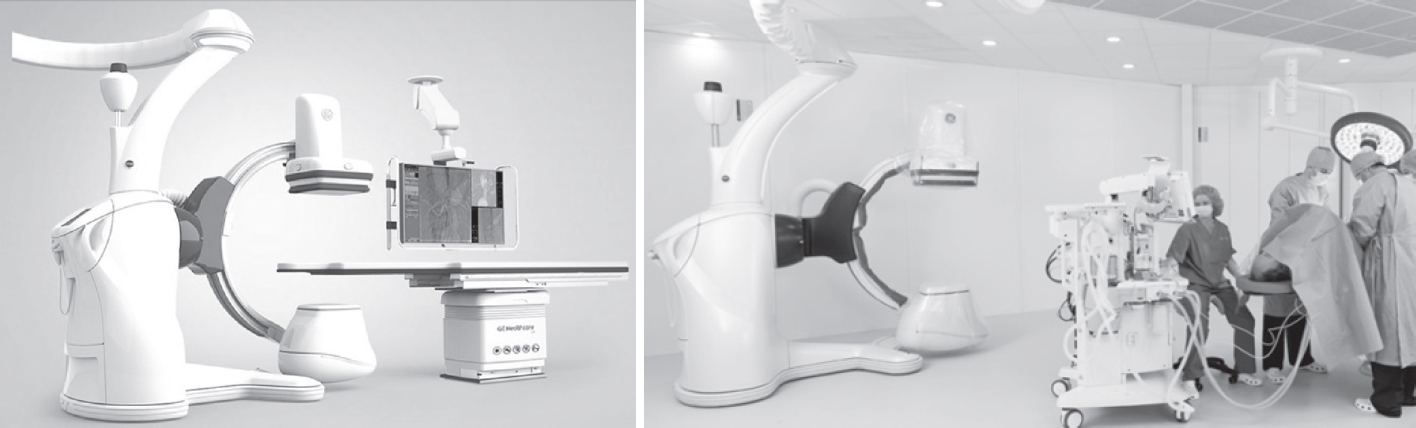
\includegraphics[width=.8\linewidth]{images/ccp_01}
%\captionof{figure}{Système d’imagerie robotisé Discovery IGS 730 en situation de travail (photo de gauche)
%et en mode parking (photo de droite)}
%\end{center}

%\begin{center}
%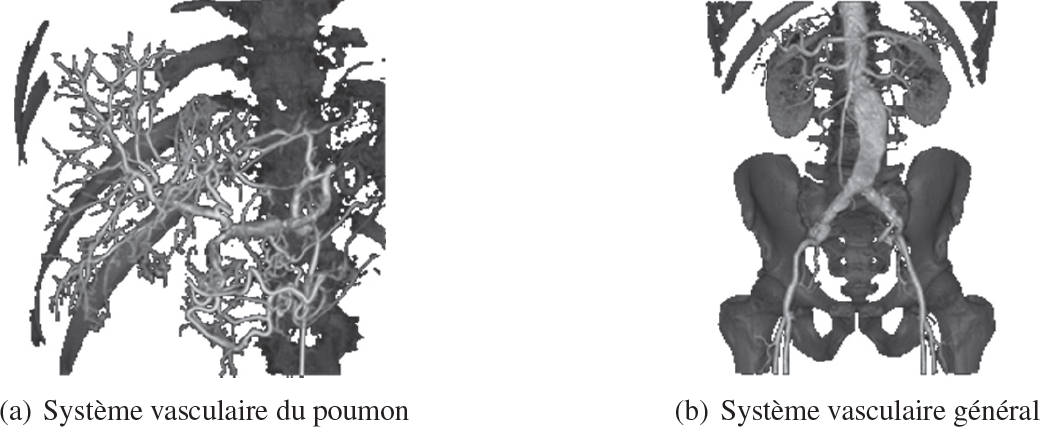
\includegraphics[width=.8\linewidth]{images/ccp_02}
%\captionof{figure}{Images 3D obtenues avec le système d’imagerie du Discovery IGS 730}
%\end{center}

%Le Discovery IGS 730 révolutionne le domaine de l’imagerie interventionnelle. Contrairement aux
%systèmes d’angiographie traditionnels, il n’est ni fixé au sol, ni suspendu au plafond, mais dispose
%d’une base motorisée guidée par laser qui transporte l’arceau d’imagerie. Cette innovation technologique
%offre une mobilité totale au système qui peut, par exemple, rejoindre de manière autonome
%une position « parking » prédéfinie afin de laisser tout le champ disponible à l’équipe médicale pour
%s’occuper du patient. Ce gain de mobilité permet également une intégration aisée en milieu clinique,
%un accès facilité au patient et des possibilités de positionnement illimitées.
%
%La figure 3 présente un extrait du cahier des charges du système d’imagerie dans la phase de vie
%d’utilisation. La figure 4 présente son diagramme de définition des blocs.
%
%\begin{center}
%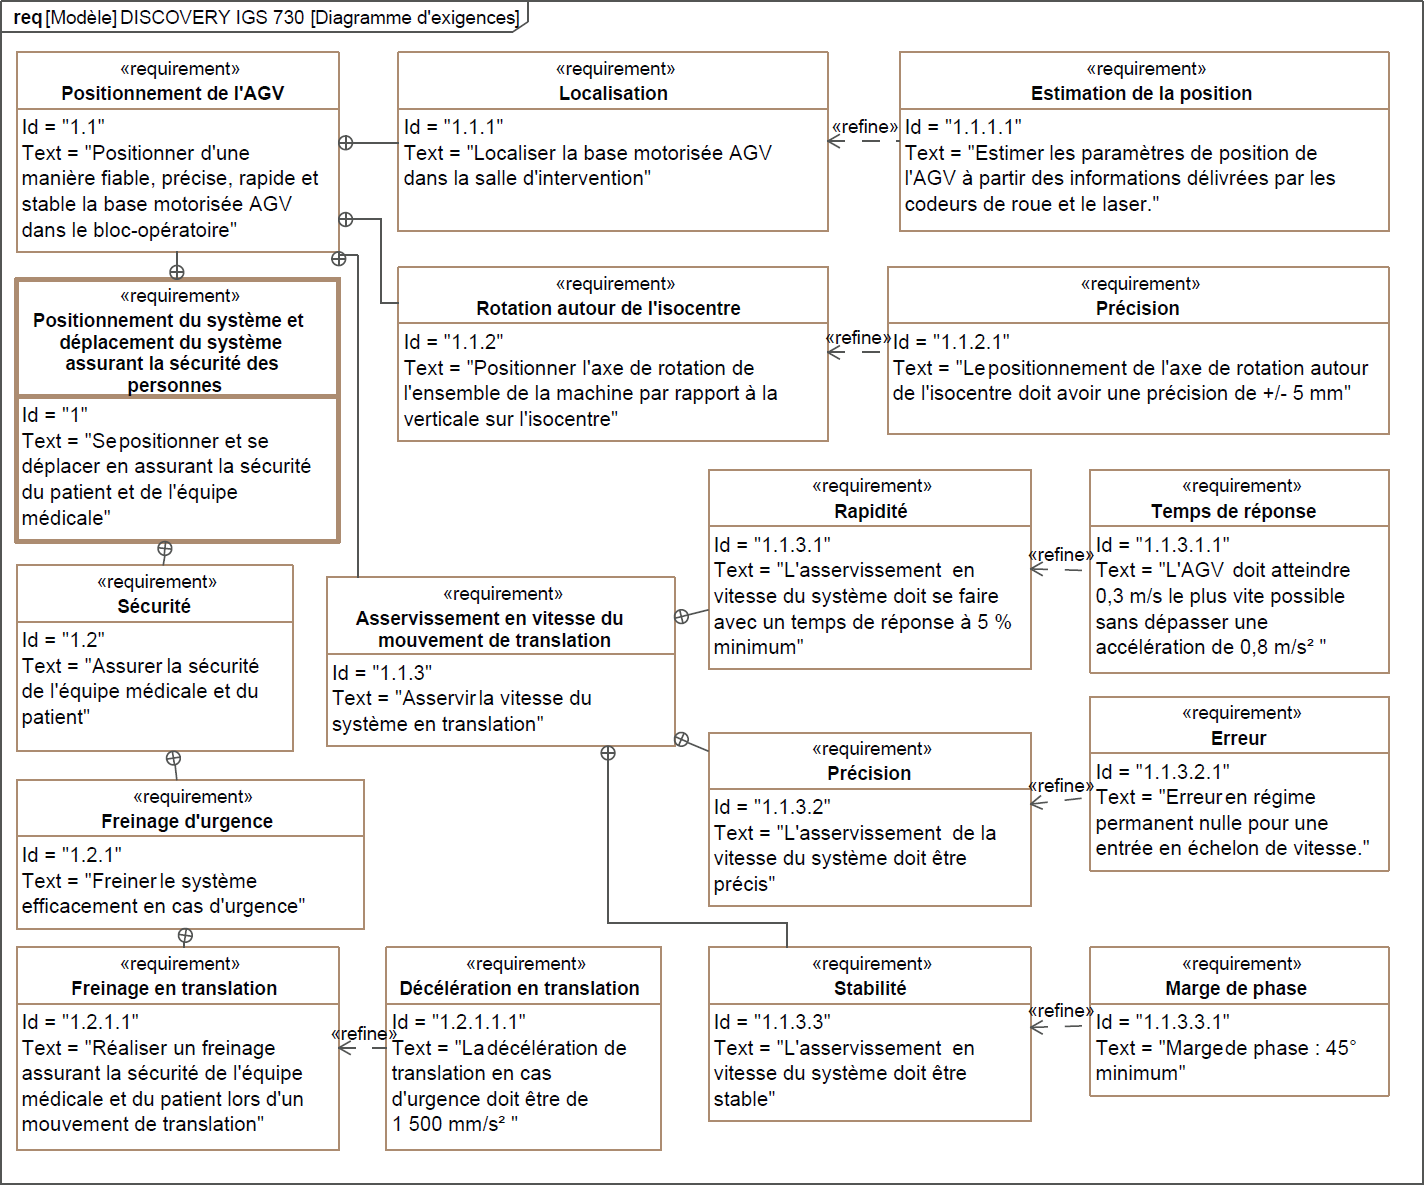
\includegraphics[width=\linewidth]{images/ccp_03}
%\captionof{figure}{Diagramme d’exigences partiel du Discovery IGS 730}
%\end{center}
%
%%
%%\begin{center}
%%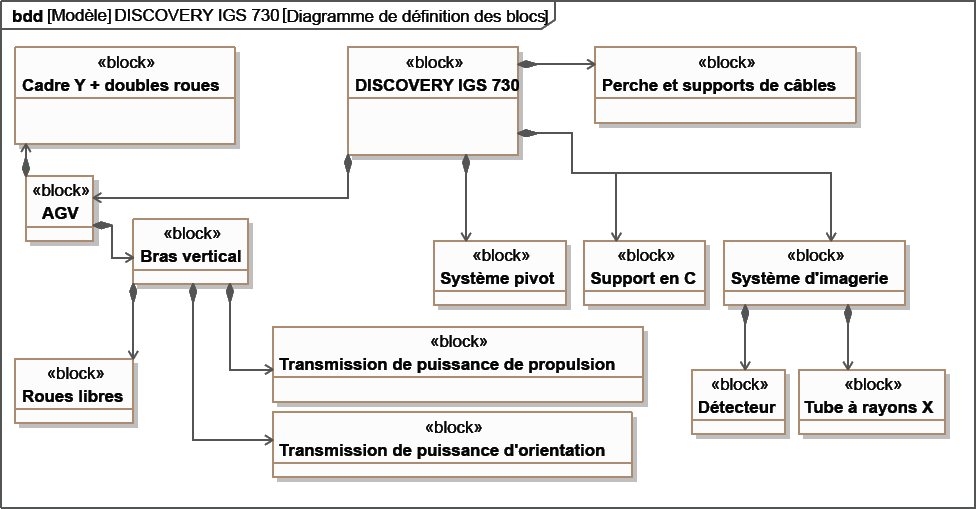
\includegraphics[width=.8\linewidth]{images/ccp_04}
%%\captionof{figure}{Diagramme de définition de blocs du Discovery IGS 730}
%%\end{center}
%%
%
%Le système Discovery IGS 730 est constitué principalement (figure 4 et figure 5) :
%\begin{itemize}
%\item d’une base motorisée, aussi appelée AGV (pour Automated Guided Vehicle, soit véhicule à
%guidage automatique) ;
%\item d’une perche et d’un support de câbles ;
%\item du sous-système d’imagerie supporté par un bras en « C » ou arceau. Le système d’imagerie
%est lié à la base motorisée par l’intermédiaire de deux liaisons pivot. Un point caractéristique
%appelé « isocentre » (point $I_C$) est rattaché au sous-système d’imagerie. Il est défini comme
%l’intersection de l’axe optique et de l’axe de la liaison pivot AGV/système pivot.
%\end{itemize}
%
%\begin{center}
%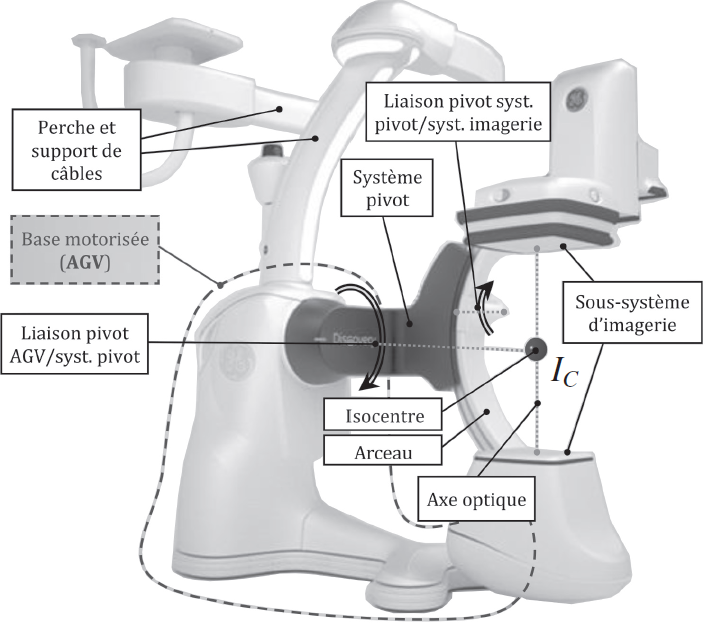
\includegraphics[width=.6\linewidth]{images/ccp_05}
%\captionof{figure}{Composants du Discovery IGS 730}
%\end{center}

La base motorisée AGV (figure \ref{fig6}) est constituée :
\begin{itemize}
\item d’une structure support, ou châssis, composée du bras vertical et du cadre Y;
\item de deux sous-ensembles roue motrice et motorisation associée (un motoréducteur d’orientation
et un motoréducteur de propulsion pour chaque roue) ;
\item de deux doubles roues « folles » non motorisées.
\end{itemize}


\begin{center}
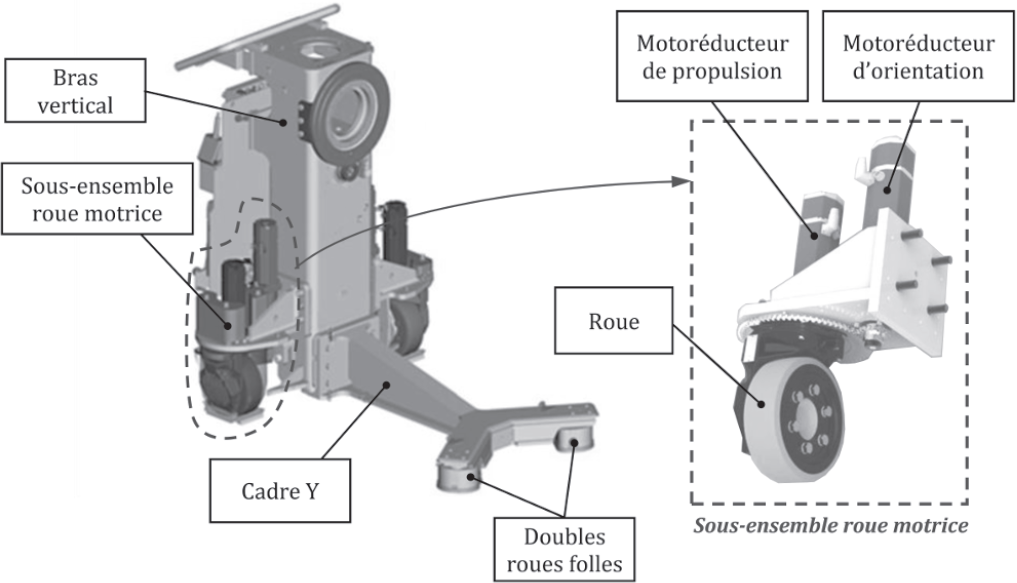
\includegraphics[width=.8\linewidth]{images/ccp_06}
\captionof{figure}{Éléments du sous-système AGV, carter et sous-système d’imagerie enlevés \label{fig6}}
\end{center}

\subsection*{Prévision des performances « l’asservissement en vitesse du mouvement de translation de
l’AGV »}

\begin{obj}
Vérifier que l’exigence d’asservissement en vitesse du mouvement de translation de la base motorisée
AGV (Id. 1.1.3) et ses sous-exigences sont respectées :
\begin{itemize}
\item 1.1.3.1.1 : l'AGV doit atteindre \SI{0,3}{m.s^{-1}} le plus rapidement possible sans dépasser une accélération de $\SI{0,8}{m.s^{-2}}$;
\item 1.1.3.2.1 : l'erreur statique doit être nulle;
\item 1.1.3.3.1 : marge de phase de 45\degres minimum.
\end{itemize}
\end{obj}
Les déplacements de la base motorisée AGV sont contrôlés de la manière suivante : au niveau de
chacun des 2 moteurs, des boucles de vitesse et de position assurent l’asservissement en vitesse et
position du système. Nous ne nous intéresserons dans le sujet qu’à la boucle de vitesse. L’objectif de
cette partie est de déterminer les paramètres de réglage de chacune des boucles d’asservissement en
vitesse lors d’un mouvement de translation de l’AGV par rapport au sol.

\subsubsection*{Étude préliminaire : moteurs brushless de propulsion}
\noindent\textbf{Hypothèses et modélisations :}
%\begin{itemize}
%\item l’AGV se déplace en ligne droite (consigne de vitesse $v_c(t)$, les roues étant dans la même
%direction que l’axe de symétrie de l’AGV) ;
%\item les roues motrices roulent sans glisser sur le sol ;
%\item la charge extérieure est supposée équi-répartie sur chacun des deux moteurs. Ainsi, pour une
%vitesse $v(t)$ de la plateforme, les deux moteurs de propulsion tournent à la même vitesse angulaire
%$\omega_m(t)$, sont alimentés par une même tension de commande $u(t)$ et fournissent un même
%couple moteur $C_m(t)$ ;
%\item les perturbations sont réparties sur chacun des axes des deux moteurs et sont modélisées par
%un même couple de perturbation équivalent appliqué sur chacun des axes moteurs $C_r(t)$ ;
%\item les caractéristiques inertielles de la plateforme sont représentées au niveau de chaque axe
%moteur par un moment d’inertie équivalent $J_{\text{eq}}$ ;
%\item 
Le comportement individuel d’un des deux moteurs brushless peut être approché par celui d’un
moteur à courant continu avec les équations électromécaniques suivantes :
$u(t)=L\dfrac{\dd i(t)}{\dd t}+Ri(t)+e(t)$, 
$C_m(t)=K_ci(t)$, 
$e(t)=K_e\omega_m(t)$, 
$C_m(t)-C_r(t)=J_{\text{eq}}\dfrac{\dd \omega_m(t)}{\dd t}$.
%\end{itemize}

On a :$R=\SI{0,07}{\ohm}$, $L=\SI{0,15}{mH}$, $K_e=\SI{0,113}{V/(rad/s)}$, 
$K_c=\SI{0,113}{Nm/A}$, $J_{\text{eq}}=\SI{5,3e-3}{kg m^2}$.
%\begin{center}
%\begin{tabular}{|c|p{3cm}|c|}
%\hline
%Symbole & Désignation & Valeurs, unités \\ \hline
%$u(t)$ &Tension d’alimentation du moteur& [V] \\ \hline
%$e(t)$ &Tension contre-électromotrice dans un moteur &[V] \\ \hline
%$i(t)$ &Intensité du courant dans un moteur& [A] \\ \hline
%$v(t)$ &Vitesse de translation du système& [m/s] \\ \hline
%$\omega_m(t)$ &Vitesse angulaire de chacun des deux moteurs &[rad/s] \\ \hline
%$C_m(t)$ & Couple moteur appliqué par chacun des deux moteurs &[N.m]\\ \hline
%$C_r(t)$ & Couple de perturbation équivalent appliqué à chacun des deux axes moteurs &[N.m]\\ \hline
%$R$ & Résistance de l’induit d’un moteur &\SI{0,07}{\ohm} \\ \hline
%$L$ & Inductance de l’induit d’un moteur &\SI{0,15}{mH }\\ \hline
%$K_e$  &Constante de vitesse d’un moteur &\SI{0,113}{V/(rad/s)} \\ \hline
%$K_c$  &Constante de couple d’un moteur &\SI{0,113}{Nm/A}\\ \hline
%$J_{\text{eq}}$  & Inertie équivalente de la moitié du système ramenée sur l’axe d’un moteur&\SI{5,3e-3}{kg m^2}\\ \hline
%\end{tabular}
%\end{center}


\subsubsection*{Fonction de transfert d’un moteur de propulsion}

On note $\Omega_m(p)$, $U(p)$, $E(p)$, $I(p)$, $C_m(p)$ et $C_r(p)$ les transformées de Laplace respectives de $\omega_m(t)$, $u(t)$, $e(t)$, $i(t)$, $C_m(t)$ et $C_r(t)$.


\subparagraph{}
\textit{Déterminer les transformées de Laplace des équations du moteur définies
en considérant des conditions initiales nulles. Compléter le schéma-blocs du document
réponse par les transmittances manquantes.}
\ifprof
\begin{corrige}
\end{corrige}
\else
\fi


\subparagraph{}
\textit{Déterminer les expressions littérales des fonctions de transfert du moteur en poursuite $H_1(p)=\left.\dfrac{\Omega_m(p)}{U(p)}\right|_{C_r(p)=0}$ (sans perturbation) et en régulation $H_2(p)=\left.\dfrac{\Omega_m(p)}{U(p)}\right|_{U(p)=0}$}
\ifprof
\begin{corrige}
\end{corrige}
\else
\fi

Le système est étudié en l’absence de perturbation, $C_r(t) = 0$.


\subparagraph{}
\textit{Réaliser l’application numérique de la fonction de transfert du moteur $\dfrac{\Omega_m(p)}{U(p)}$
et mettre le résultat sous la forme : $\dfrac{K}{\left(1+\tau_1 p\right)\left(1+\tau_2 p\right)}$.}
\ifprof
\begin{corrige}
\end{corrige}
\else
\fi
\subsection*{Étude de l’asservissement en vitesse de la base motorisée AGV}

Pour une consigne de vitesse $v_c(t)$ [m/s], les microcontrôleurs de pilotage génèrent une tension de
consigne de rotation à appliquer à chaque moteur $u_c(t)$ [V]. Un traitement numérique de la vitesse
relevée sur l’axe de chaque moteur fournit une tension mesurée $u_m(t)$ [V], image de la vitesse de
rotation du moteur $\omega_m(t)$. Un correcteur (défini par la suite) adapte le signal écart entre la tension de
consigne et la tension mesurée, ce qui permet après correction et amplification, de définir la tension
d’alimentation $u(t)$ à appliquer aux moteurs.


\begin{center}
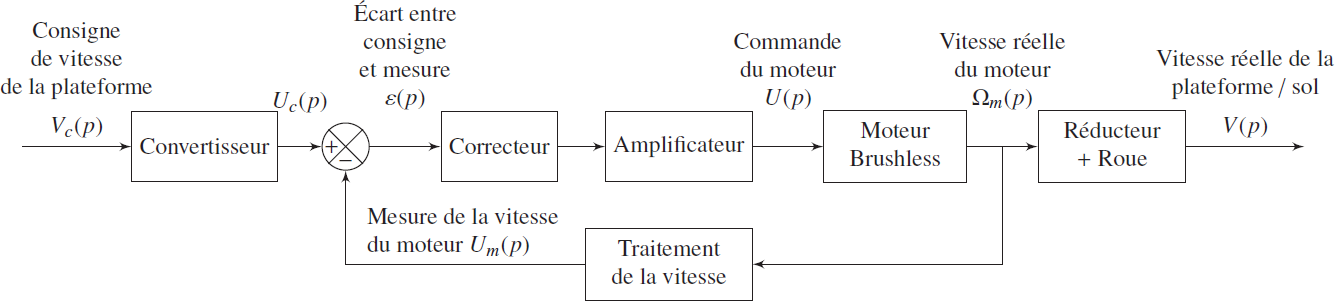
\includegraphics[width=\linewidth]{images/ccp_08}
\captionof{figure}{Schéma-blocs fonctionnel de l’asservissement en vitesse d’un des deux moteurs}
\end{center}


\begin{center}
\begin{tabular}{|p{3cm}|c|}
\hline
Blocs & Fonctions de transfert  \\ \hline
Convertisseur & $K_\text{conv}$ (à déterminer) \\ \hline
Correcteur & $C(p)$ (réglé par la suite) \\ \hline
Amplificateur & $K_A = 7,9$ sans unité \\ \hline
Traitement numérique de la vitesse & $K_{\text{Vit}}= \SI{1,4e-3}{V/(rad/s)}$ \\ \hline
Réduction et roue & $K_R$ (à déterminer) \\
\hline
\end{tabular}
\end{center}
Indépendamment des résultats trouvés précédemment, la fonction de transfert du moteur brushless
sera prise égale à :  $H_m(p)=\dfrac{K_m}{\left(1+\tau_1 p\right)\left(1+\tau_2 p\right)}$, avec $K_m=8,85$, $\tau_1=\SI{0,027}{s}$ et $\tau_2=\SI{0,0023}{s}$.

Le moteur est suivi d’un réducteur à deux étages : le premier avec un rapport de réduction $k_1 = \dfrac{1}{4}$ et le second avec un rapport de réduction $k_2 = \dfrac{1}{28,9}$. Le rayon $r$ des roues motrices est de $\SI{115}{mm}$.

\subparagraph{}
\textit{Déterminer les valeurs numériques et unités SI des gains $K_R$ (ensemble réducteur et roue) et
$K_{\text{conv}}$ (convertisseur) en sachant que lorsque la vitesse réelle de l’AGV $v(t)$ est égale à la vitesse
de consigne $v_c(t)$, l’écart $\varepsilon (t)$ doit être nul.}
\ifprof
\begin{corrige}
\end{corrige}
\else
\fi
%
%\subparagraph{}
%\textit{Compléter le schéma-bloc sur le document réponse DR2 en y faisant figurer les fonctions de
%transfert sous forme littérale dans le domaine de Laplace avec des conditions initiales nulles,
%ainsi que les signes des sommateurs.
%}
\subparagraph{}
\textit{Réaliser le schéma-blocs en y faisant figurer les fonctions de
transfert sous forme littérale dans le domaine de Laplace avec des conditions initiales nulles,
ainsi que les signes des sommateurs.
}
\ifprof
\begin{corrige}
\end{corrige}
\else
\fi

\subsection*{Étude du système non corrigé : $C(p)=1$}
\subparagraph{}
\textit{Déterminer, en fonction notamment de $K_m$, $K_A$, $K_{\text{vit}}$, $\tau_1$ et $\tau_2$, l'expression de la fonction de transfert de la boucle de vitesse sous la forme canonique d'un système du second ordre $H(p)=\dfrac{V(p)}{V_c(p)}=\dfrac{K}{1+\dfrac{2\xi}{\omega_0}p+\dfrac{p^2}{\omega_0^2}}$. Donner les expressions littérales et numériques de $K$, $\xi$ et $\omega_0$. }

%\subparagraph{}
%\textit{Justifier que l’accélération maximum peut être approchée par $a_{\text{max}}=\dfrac{V_{\text{max}}}{t_{5\%}}$.}
%\ifprof
%\begin{corrige}
%\end{corrige}
%\else
%\fi

On considère que l'accélération maximum peut être approchée par $a_{\text{max}}=\dfrac{V_{\text{max}}}{t_{5\%}}$.

\subparagraph{}
\textit{À l’aide de l’abaque du document réponse, déterminer le temps de réponse à 5\% de la
boucle de vitesse (faire apparaître les tracés sur le document réponse). Ce temps de réponse est-il
satisfaisant vis-à-vis de l’exigence Id. 1.1.3.1.1 ? Sinon, comment satisfaire cette exigence ?}
\ifprof
\begin{corrige}
\end{corrige}
\else
\fi

\subparagraph{}
\textit{Déterminer l’erreur en régime permanent de la boucle de vitesse pour une entrée en échelon.
Permet-elle de satisfaire l’exigence Id. 1.1.3.2.1 ? Sinon, comment satisfaire cette exigence ?}
\ifprof
\begin{corrige}
\end{corrige}
\else
\fi

\subsection*{Étude du système non corrigé : $C(p)=K_P\left(1+\dfrac{1}{T_i p}\right)$}

\subparagraph{}
\textit{Déterminer, en fonction notamment de $K_m$, $K_A$, $K_{\text{vit}}$, $\tau_1$, $\tau_2$, l'expression de la fonction de transfert en boucle ouverte, sous la forme canonique suivante : $H_{\text{BO}}(p)=\dfrac{K_{\text{BO}}\left(T_i p +1 \right)}{p\left(1+\tau_1 p \right)\left(1+\tau_2 p \right)}$. Donner l'expression littérale de $K_{\text{BO}}$.}
\ifprof
\begin{corrige}
\end{corrige}
\else
\fi


\subparagraph{}
\textit{On choisit $T_i$ de façon à compenser le "mode le plus lent". Donner la valeur de $T_i$.}
\ifprof
\begin{corrige}
\end{corrige}
\else
\fi

L’exigence de stabilité Id. 1.1.3.3.1 impose une marge de phase de 45\degres. Indépendamment de la réponse à la question précédente, on prendra $K_{\text{BO}} = 37 K_p$.

\subparagraph{}
\textit{Ce correcteur permet-il de répondre à l’exigence de précision ? Tracer les asymptotes et les
courbes réelles avec $K_p = 1$ dans le plan de Bode du document réponse. Déterminer le
gain $K_p$ du correcteur permettant de satisfaire l’exigence de stabilité en étant le plus rapide (on
s’intéressera à la bande passante à \SI{0}{dB}).}
\ifprof
\begin{corrige}
\end{corrige}
\else
\fi

La figure du document réponse présente sur un même graphe les réponses à une consigne en
échelon d’amplitude \SI{0,3}{m/s} obtenues par simulation pour différentes valeurs de $K_p$.


\subparagraph{}
\textit{Choisir le gain $K_p$, parmi les trois valeurs proposées, satisfaisant l’exigence de stabilité et de
rapidité (notamment l’accélération qui ne doit pas dépasser \SI{0,8}{m.s^{-2}}). Appuyez votre réponse
par des tracés sur le document réponse.}
\ifprof
\begin{corrige}
\end{corrige}
\else
\fi


\subsection*{Synthèse}
\subparagraph{}
\textit{Les courbes du document réponse représentent la réponse réelle relevée sur la base
motorisée AGV et le résultat obtenu par simulation numérique pour une entrée en échelon
d’amplitude \SI{0,3}{m/s}. Comparer quantitativement les résultats au cahier des charges et conclure
sur les écarts.}
\ifprof
\begin{corrige}
\end{corrige}
\else
\fi


\begin{center}
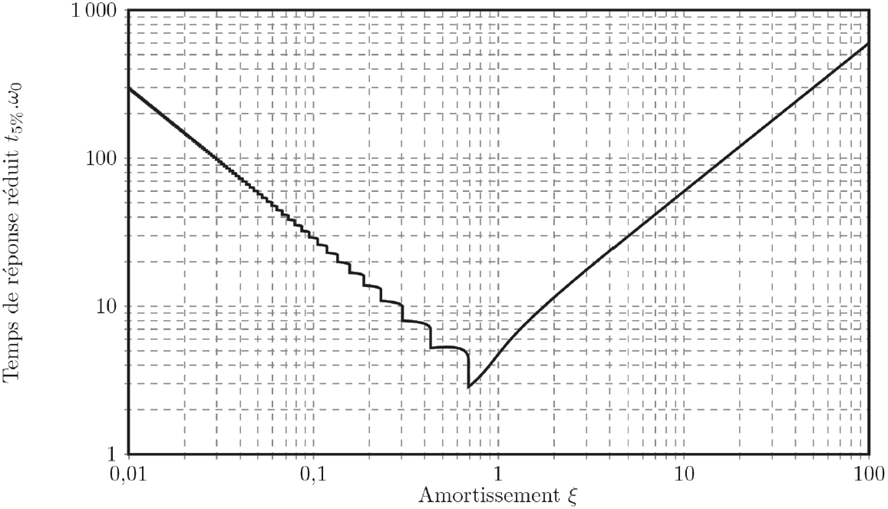
\includegraphics[width=\linewidth]{images/ccp_09}
\end{center}


\begin{center}
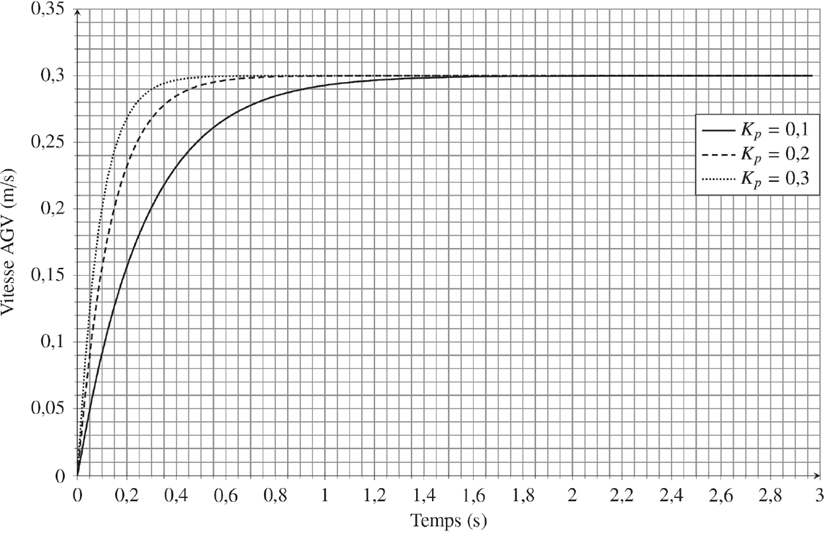
\includegraphics[width=\linewidth]{images/ccp_10}
\end{center}


\begin{center}
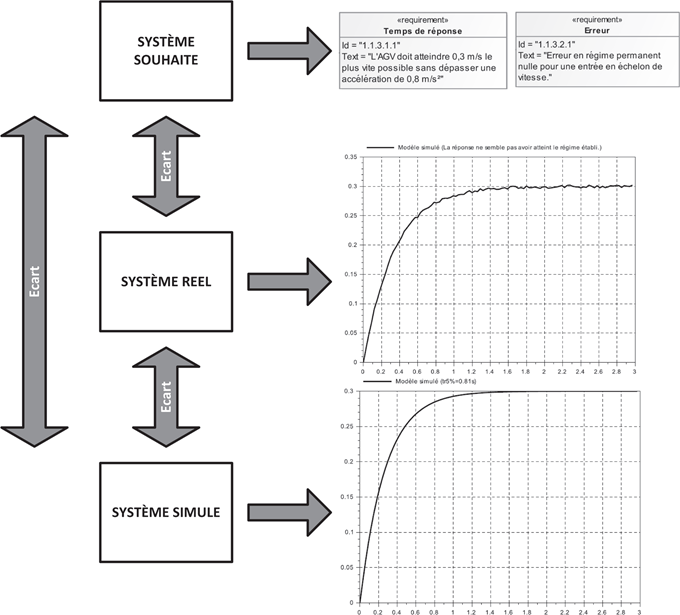
\includegraphics[width=\linewidth]{images/ccp_11}
\end{center}







%%%%%%%%%%%%%%%%%%%%%%%%%%%%%%%%%%%%%%%%%%%%%%%%%%%

\ifprof
\end{multicols}
\else
\end{multicols}
\fi


\ifprof
\else


\begin{center}
%\includegraphics[width=\linewidth]{ecart}
%\textit{}
\end{center}

\begin{center}
%\includegraphics[width=.9\linewidth]{PositionQuille}
\end{center}


\fi
%
%\end{document}
%
%\subparagraph{}\textit{}
%\ifprof
%\begin{corrige}
%\end{corrige}
%\else
%\fi
%
%\begin{center}
%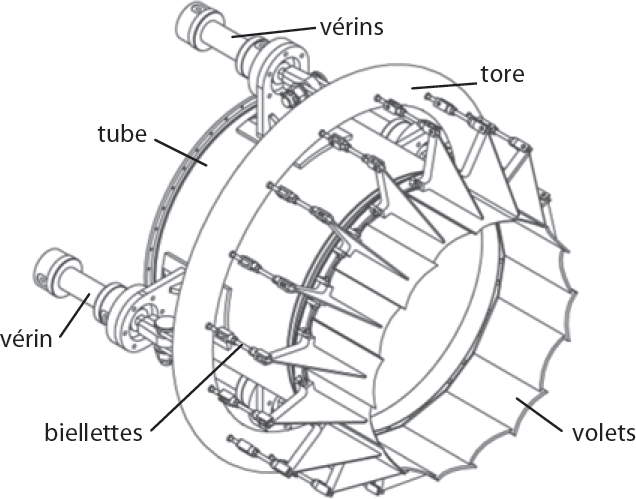
\includegraphics[width=\linewidth]{fig_04}
%%\textit{}
%\end{center}

